% !TEX root = ../../CompVis.tex
\section{Model Fitting}
Find a high-level explanation (model) that well explains the low-level obersvations (edges).

\subsection{Voting Algorithms}
\begin{enumerate}
    \item Every feature casts votes for all models that are compatible with it
    \item Choose models that accumulated a lot of votes
\end{enumerate}

\subsubsection{Hough Transform}
\begin{minipage}[t]{0.5\textwidth}
    Advantages
    \begin{itemize}
        \item All points are processed independently, so the algorithm can cope with occlusions and gaps
        \item Voting algorithms are robust to clutter, because points not corresponding to any model are unlikely to contribute consistently to any single bin
        \item Can detect multiple instances of a model in a single pass
    \end{itemize}
\end{minipage}
\begin{minipage}[t]{0.5\textwidth}
    Disadvantages
    \begin{itemize}
        \item Only suitable for models with few parameters
        \item Must filter out spurious peaks in hough accumulator
        \item Quantization of Hough space is tricky
    \end{itemize}
\end{minipage}

\paragraph{Line}
Parametrize line so it's parameters are bounded: $d = x\cos\theta - y\sin\theta$
\lstinputlisting{sections/ModelFitting/src/hough_line.pseudo}
How large are the bins in the accumulator?
\begin{itemize}
    \item To small: Many weak peaks due to noise
    \item To large: Poor accuracy in locating the line. Many votes from clutter might end up in the same bin
    \item Just right: One strong peak per line, despite noise
\end{itemize}
Extensions
\begin{itemize}
    \item Extension 1: Make sure an edge pixel only votes for lines thath have (almost) the direction of the edge (orthogonal to gradient)
    \item Extension 2: If a line is chosen, look for groups of edge points that voted for that line $\rightarrow$ find start point and end point of segment
\end{itemize}

\paragraph{Circle}
\begin{minipage}{0.48\textwidth}
    Parametrize circle so it's parameters are bounded:\\ $(x-a)^2 + (y-b)^2 = r^2$.
    Circle with center $(a,b)$ and radius $r$. $\rightarrow$ 3D voting space.

    \lstinputlisting{sections/ModelFitting/src/hough_circle.pseudo}
\end{minipage}
\begin{minipage}{0.52\textwidth}
    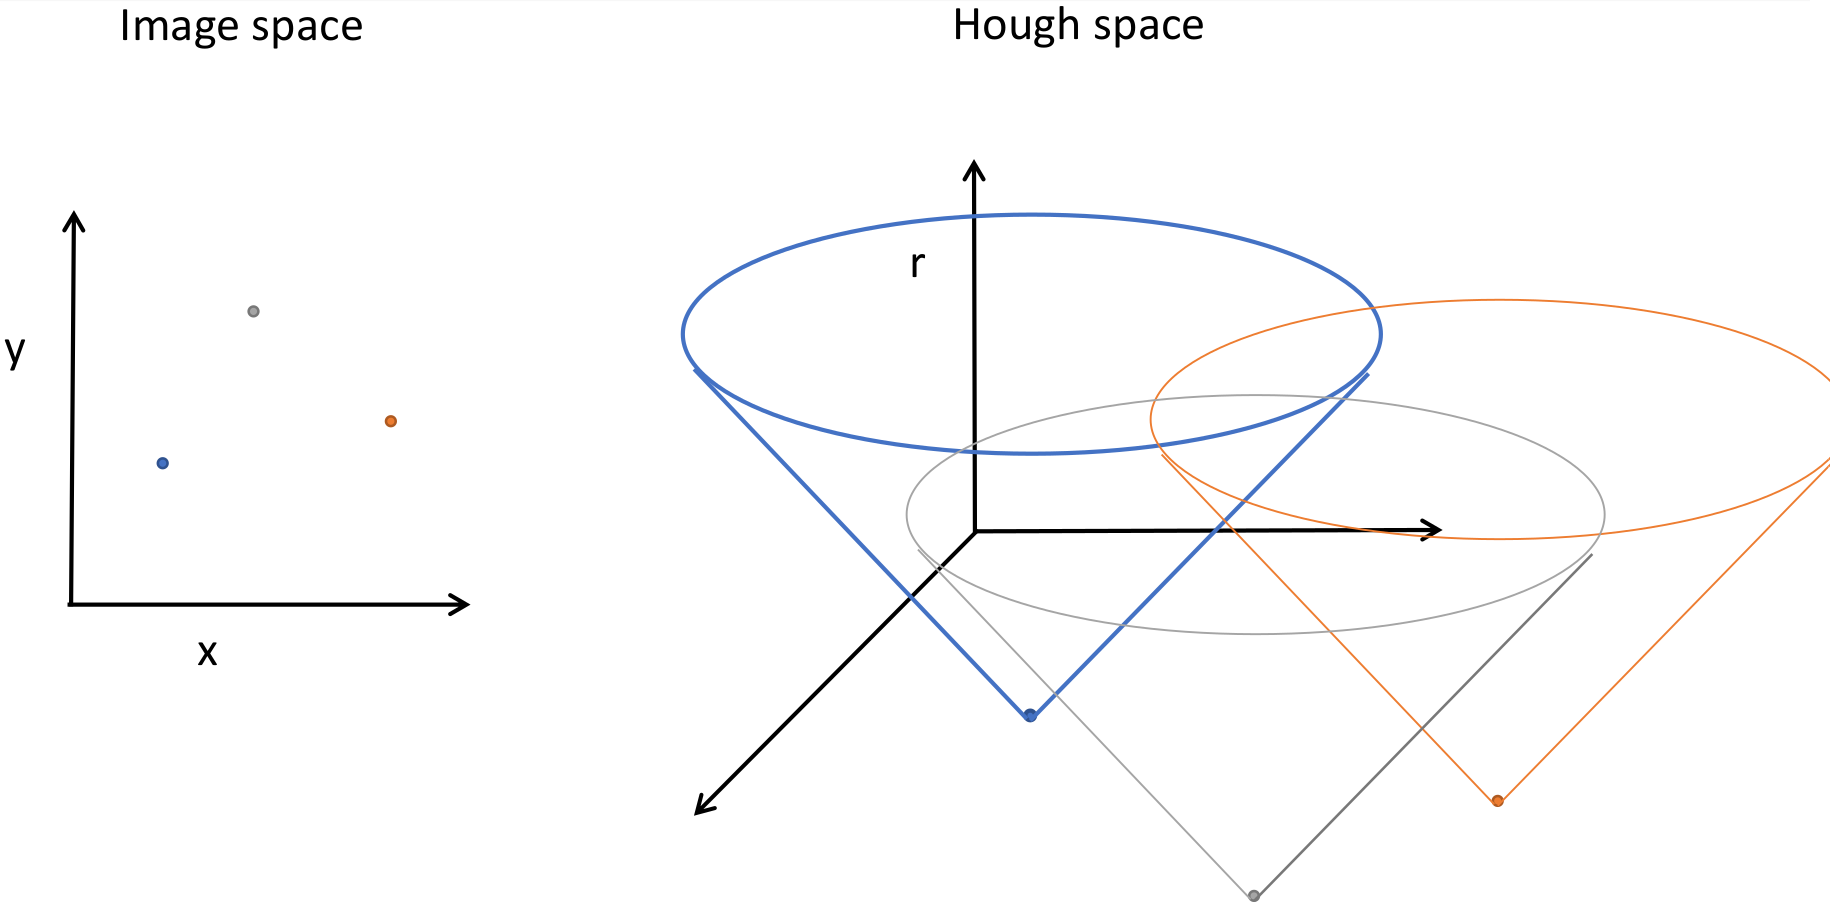
\includegraphics[width=1\textwidth]{sections/ModelFitting/img/circle_space.png}
\end{minipage}